\documentclass{beamer}
\mode<presentation> {
%\usetheme{Madrid}
%\usetheme{default}
\usepackage{color}
\definecolor{bottomcolour}{rgb}{0.21,0.11,0.21}
\definecolor{middlecolour}{rgb}{0.21,0.11,0.21}
\setbeamercolor{structure}{fg=white}
\setbeamertemplate{frametitle}[default]%[center]
\setbeamercolor{normal text}{bg=black, fg=white}
\setbeamertemplate{background canvas}[vertical shading]
[bottom=bottomcolour, middle=middlecolour, top=black]
\setbeamertemplate{items}[circle]
\setbeamertemplate{navigation symbols}{} %no nav symbols
\setbeamercolor{block title}{use=structure,fg=white,bg=structure.fg!50!red!50!blue!100!green}
\setbeamercolor{block body}{parent=normal text,use=block title,bg=block title.bg!5!white!10!bg,fg=white}
\setbeamertemplate{navigation symbols}{}
}
\usepackage{graphicx} 
\usepackage{booktabs} 
\usepackage[utf8]{inputenc}  
\usepackage[T1]{fontenc}  
\usepackage{geometry}     
%\usepackage[francais]{babel} 
\usepackage{eurosym}
\usepackage{verbatim}
\usepackage{ragged2e}
\justifying
\input{cc_beamer}
\title[Firefox OS par Mozilla]{Firefox OS par Mozilla} 
\author{Le Printemps de l'Entreprise - IUT de Vannes}
\author{Genma}
\begin{document}
\begin{frame}
	\titlepage
	\begin{center}		
	\includegraphics[scale=0.2]{./images/firefox-os.jpg}
		\\	
	\CcGroupByNcSa{0.83}{0.95ex}\\[2.5ex]
		{\tiny\CcNote{\CcLongnameByNcSa}}
		\vspace*{-2.5ex}
	\end{center}
\end{frame}

\begin{frame}
\frametitle{\includegraphics[scale=0.4]{./images/Genma.jpg} \ \ \  A propos de moi  }
\begin{columns}[c] 
\column{.55\textwidth} 
\textbf{Où me trouver sur Internet?}
\begin{itemize}
\item Le Blog de Genma : http://genma.free.fr
\item Twitter : http://twitter.com/genma
\end{itemize}

\column{.5\textwidth} 
\includegraphics[width=5cm,height=5cm]{./images/blog.png} 
\end{columns}
\end{frame}

%----------------------------------------------------------------------------------------
\begin{frame}
\frametitle{Remerciements}
\justifying{
Je remercie la communauté francophone autour de Firefox OS pour les builds communautaires 
\url{http://builds.firefoxos.mozfr.org/}
le support, les billets de blog, la promotion de FFOS.\\
Ainsi que Mozilla pour avoir lancé FFOS.
}
\end{frame}
%----------------------------------------------------------------------------------------
\begin{frame}
\begin{center}
\Huge{Introduction}
\\~\\
\includegraphics[scale=0.3]{./images/firefox-os.jpg}
\end{center}
\end{frame}

\begin{frame}
\frametitle{Mozilla - De Firefox à FirefoxOS}
\justifying{
En 2004, Mozilla a lancé Firefox, le navigateur web gratuit et
désintéressé pour votre ordinateur.
\\~\\
En 2014, Mozilla introduit en France Firefox OS, le système d’
exploitation respectueux de votre vie privée pour votre téléphone.
\\~\\
En 2016, Mozilla choisit de réorienter Firefox OS vers l'I.O.T. (Internet des Objets)
}
\end{frame}
%---------------------------------------------------------------------------------------
\begin{frame}
\frametitle{FirefoxOS - un OS libre}
\justifying{
Firefox OS est conçu par une communauté internationale de bénévoles, et de développeurs situés dans plusieurs pays, notamment dans les bureaux de Mozilla Paris.
\\~\\
Le logiciel est libre : Firefox OS est un logiciel libre, sans secrets, auditable. Tout le code source est ouvert et disponible.
}
\end{frame}

%----------------------------------------------------------------------------------------
\begin{frame}
\begin{center}
\Huge{Architecture}
\\~\\
\includegraphics[scale=0.3]{./images/firefox-os.jpg}
\end{center}
\end{frame}
%---------------------------------------------------------------------------------------
\begin{frame}
\frametitle{Architecture de FFOS}
\begin{center}
\includegraphics[scale=0.3]{./images/ffos_architecture.jpg}
\end{center}
\end{frame}

\begin{frame}
\begin{center}
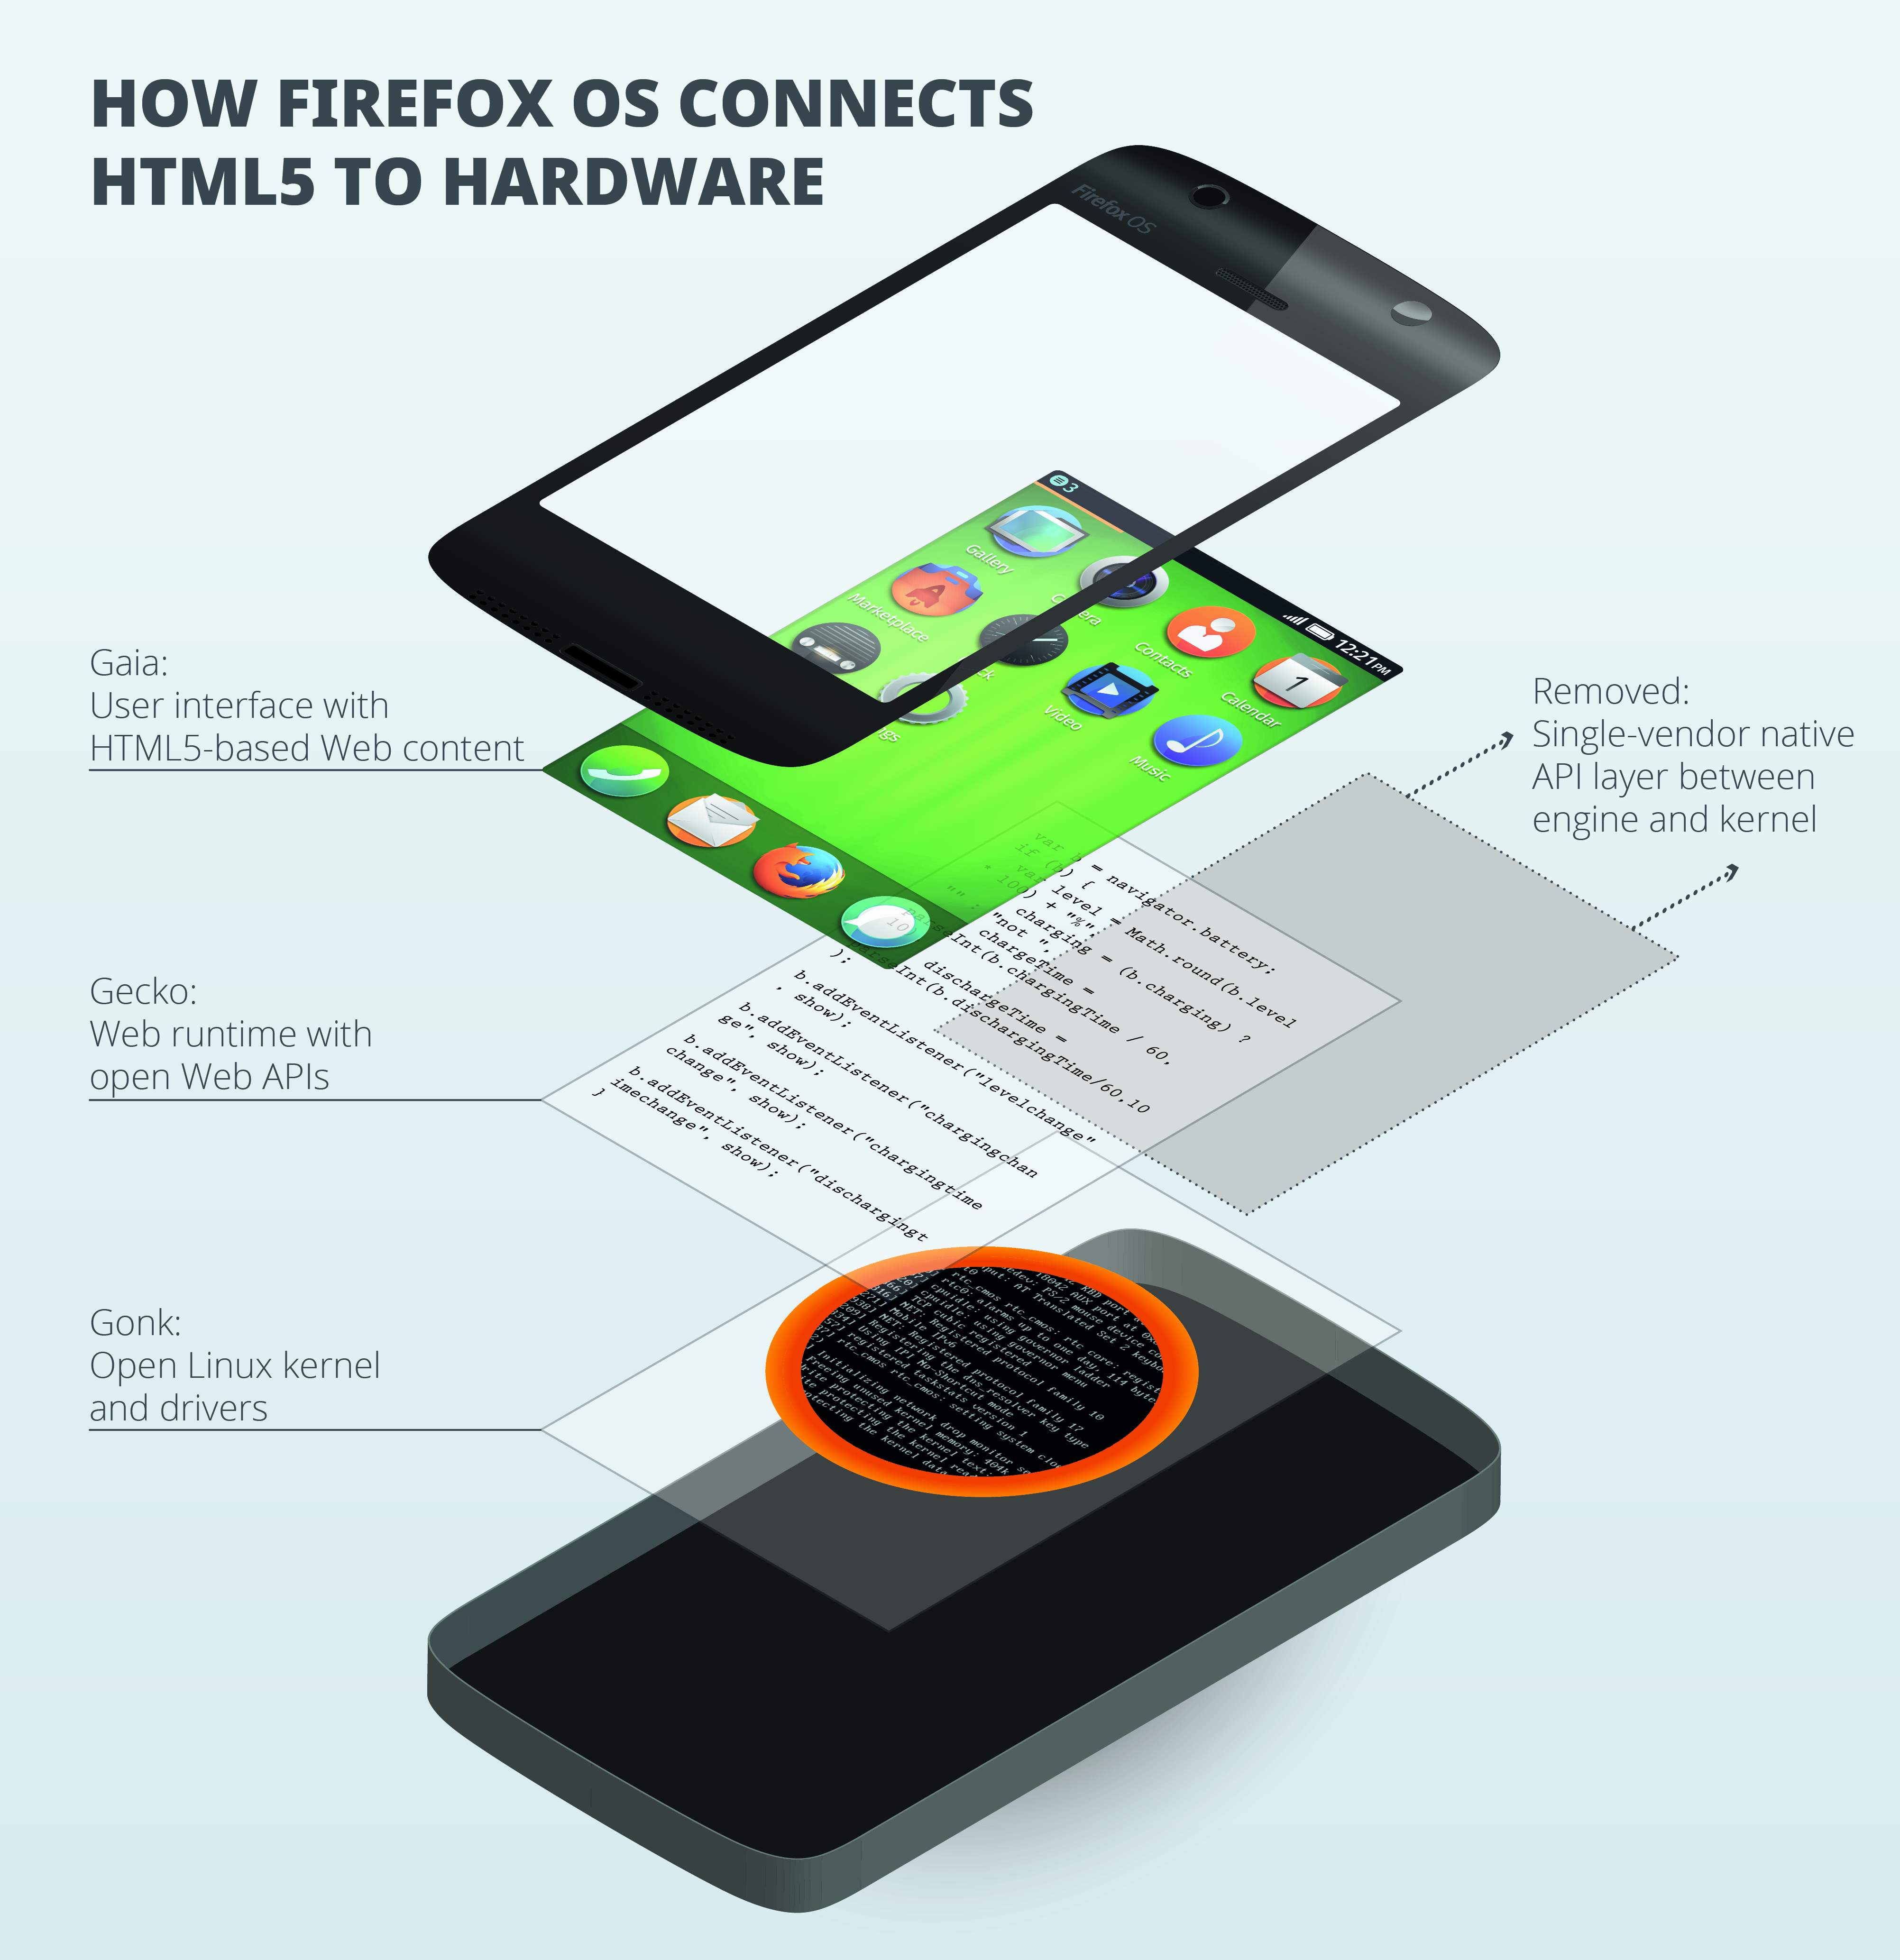
\includegraphics[scale=0.06]{./images/Firefox_Layers.jpg}
\end{center}
\end{frame}
%---------------------------------------------------------------------------------------
\begin{frame}
\frametitle{Architecture de FFOS}
\begin{block}{Gaia - l'interface}
\justifying{Gaia a le rôle d'interface utilisateur de Firefox OS et contrôle tout ce qui interagit avec l'écran.}
\end{block}
\begin{block}{Gecko - le moteur}
\justifying{
Gecko est l'application permettant d'exécuter Firefox OS. Il permet le support des trois standards : HTML, CSS et JavaScript.}
\end{block}
\begin{block}{Gonk - le noyau}
\justifying{Gonk consiste en un noyau Linux et une couche d'abstraction matérielle de l'espace utilisateur (HAL).}
\end{block}
\end{frame}

\begin{frame}
\frametitle{Les appplications pour FFOS}
Les applications sont toutes en HTML5/CSS3/Javascript
\begin{itemize}
\item N'importe qui peut en développer une.
\item Toutes ne sont pas libres.
\end{itemize}

\begin{center}
\includegraphics[scale=0.3]{./images/logo-html5.jpg} 
\end{center}
\end{frame}


%----------------------------------------------------------------------------------------
\begin{frame}
\begin{center}
\Huge{Quel matériel?}
\\~\\
\includegraphics[scale=0.3]{./images/FirefoxOS-logo_610x385.png}
\end{center}
\end{frame}
%---------------------------------------------------------------------------------------
\begin{frame}
\frametitle{Les smartphones compatibles}
\begin{block}{Firefox OS est compatible avec un certain nombre d'appareils}
\justifying{Sony Xperia Z3, Z3c, Samsung Nexus S, le Samsung Nexus S 4G, le Samsung Galaxy S II, le Samsung Galaxy Nexus, le Nexus 4 et d'autres.
}
\\
\url{https://hacks.mozilla.org/2015/10/build-and-run-firefox-os-on-sony-open-devices/}
\end{block} 
\end{frame}

%----------------------------------------------------------------------------------------
\begin{frame}
\frametitle{Des smartphones à l'I.O.T.}
Décembre 2015: Mozilla annonce la réorientation du projet Firefox OS vers les objets connectés (I.O.T.).
\\~\\
Mars 2015 : Mozilla s’engage dans un plan de transition de Firefox OS pour smartphone vers un projet open source dirigé par une communauté de contributeurs bénévoles. Mozilla investira des ressources dans la transition pour qu’elle soit au final un succès.
\\~\\
Le projet lui sera nommé B2G OS pour smartphones jusqu’à ce que la direction communautaire bénévole du projet lui trouve un meilleur nom.
\end{frame}

%----------------------------------------------------------------------------------------
\begin{frame}
\begin{center}
\Huge{Mozilla et I.O.T.}
\\~\\
\includegraphics[scale=0.3]{./images/firefox_os_connected_devices_leak.png}
\end{center}
\end{frame}

%---------------------------------------------------------------------------------------
\begin{frame}
\frametitle{Avancée dans le domaine des objets connectés}
\begin{block}{Projet Link}
\justifying{
votre agent personnel qui sait comment vous souhaitez interagir avec vos objets connectés chez vous, et automatise leur usage. Tout cela se fait de façon sécurisée et sous votre contrôle.}
\end{block} 

\begin{block}{Projet Sensor Web }
\justifying{Le chemin le plus facile entre les capteurs et les données, pour que les contributeurs puissent construire ensemble une vision compréhensive de leurs environnements. Nous lançons un projet pilote pour construire un réseau de capteurs pm2.5 sur la base du crowdsourcing.}
\end{block} 
\end{frame}

%---------------------------------------------------------------------------------------
\begin{frame}
\frametitle{Avancée dans le domaine des objets connectés}
\begin{block}{Projet Smart Home}
\justifying{A mi-chemin entre les solutions clé-en-main (telles qu’Apple Homekit) et celles à construire soi-même (telles que Raspberry Pi). Combinant du matériel modulaire et abordable avec des règles faciles d’utilisation, Smart Home fournit aux individus la capacité de résoudre les problèmes du quotidien de façon nouvelle et créative.
}
\end{block} 

\begin{block}{Projet Vaani}
\justifying{Un kit dédié à l’Internet des Objets à l’intention des développeurs, constructeurs et autres utilisateurs souhaitant ajouter une interface voix à leurs appareils de façon flexible et personnalisable. Nous allons prochainement tester les interactions avec la maison pour ensuite accéder à ces services via un Web ouvert.
}
\end{block} 
\end{frame}

%---------------------------------------------------------------------------------------
\begin{frame}
\frametitle{Les télévisions}
\begin{block}{Panasonic TX-65CR852}
\begin{center}
\includegraphics[scale=0.38]{./images/firefox_os_tv.jpg}
\end{center}
\end{block} 
\end{frame}

%----------------------------------------------------------------------------------------
\begin{frame}
\begin{center}
\Huge{Où trouver des informations \\ sur FFOS?}
\end{center}
\end{frame}

\begin{frame}
\frametitle{Où trouver des informations sur FFOS?}
\begin{itemize}
\item Le site officiel par Mozilla \url{https://www.mozilla.org/fr/firefox/os/}
\item Le forum de Mozilla-fr \url{https://forums.mozfr.org}
\item Les mailing-listes \url{http://mozfr.org/participer}
\item Bugzilla \url{https://bugzilla.mozilla.org}
\item Les blogs de la communauté \url{http://mozfr.org}
\item Twitter/Diaspora-Framasphère via \#FirefoxOS
\end{itemize}
\end{frame}

%----------------------------------------------------------------------------------------
\begin{frame}
\begin{center}
\Huge{Contribuer à FFOS?}
\\~\\
\includegraphics[scale=0.3]{./images/firefox-os.jpg}
\end{center}
\end{frame}

%----------------------------------------------------------------------------------------
\begin{frame}
\frametitle{Développer pour FFOS}

\begin{block}{La documentation - liens}
\begin{itemize}
\item \url{https://developer.mozilla.org/fr/docs/Mozilla/Boot_to_Gecko/Writing_apps_for_Boot_to_Gecko}
\item \url{https://developer.mozilla.org/en-US/docs/Mozilla/Firefox_OS}
\item \url{https://wiki.mozilla.org/B2G/Hacking}
\item \url{https://developer.mozilla.org/en/Firefox_OS/Developing_Gaia}
\end{itemize}
\end{block}

\begin{block}{Regarder les applications existantes}
\justifying{
Il est possible de télécharger des applications existantes et de regarder leur code source, pour apprendre, comprendre...
}
\end{block}

\begin{block}{Contribuer au code source de FFOS}
\justifying{
Tout le code source est disponible sur Github.
}
\end{block}
\end{frame}

%---------------------------------------------------------------------------------------
\begin{frame}
\begin{center}
\Huge{Questions et discussion}
\\~\\
\includegraphics[scale=0.3]{./images/firefox-os.jpg}
\end{center}
\end{frame}

%======================================================
\begin{frame}
\begin{center}
\Huge{ANNEXES}
\end{center}
\end{frame}

%---------------------------------------------------------------------------------------
\begin{frame}
\frametitle{Architecture de FFOS - Détaillée 1/3}
\begin{block}{Gonk - le noyau}
\justifying{Gonk consiste en un noyau Linux et une couche d'abstraction matérielle de l'espace utilisateur (HAL)}.
\begin{itemize}
\item Couche basse
\item Kernel Linux + Matériels
\item Hardware
\item libre ou propriétaire
\item Abstraction Layer (HAL)
\item Pas exposé le JS
\item Isolé de Gaia
\item Communication par Gecko
\end{itemize}
\end{block}
\end{frame}

\begin{frame}
\frametitle{Architecture de FFOS - Détaillée 2/3}
\begin{block}{Gecko - le moteur}
\justifying{
Gecko est l'application permettant d'exécuter Firefox OS. Il permet le support  des trois standards : HTML, CSS et JavaScript}.
\begin{itemize}
\item Moteur de rendu HTML5
\item Gestion des API
\item De plus en plus complet
\item Exécution des applications (runtime)
\item Mécanisme de lancement dans Firefox pour HTML 5, CSS et Javascript
\end{itemize}
\end{block}
\end{frame}

\begin{frame}
\frametitle{Architecture de FFOS - Détaillée 3/3}
\begin{block}{Gaia - l'interface}
\justifying{Gaia a le rôle d'interface utilisateur de Firefox OS et contrôle tout ce qui interagit avec l'écran}.
\begin{itemize}
\item Interface utilisateur (IHM)
\item Construction API Full Web
\item HTML 5 + open Web
\item Communique avec Geckovia des Web API
\item Les Apps sont exécutés enmode sandbox
\item Offline
\item LocalStorage, appCache
\end{itemize}
\end{block}
\end{frame}

%---------------------------------------------------------------------------------------
\end{document}